\paragraph{}
A natural language processing (NLP) is a subfield of linguistics and computer science. In recent years many deep learning techniques have been successfully applied to many NLP problems. These are, for instance, sentiment analysis, machine translation, text classification, semantic similarity and many more \cite{nlp_devopedia}. 

\paragraph{}
A problem in the NLP is that a dimension of the space of possible words or sentences fed into a neural network is immensely high. The way how neural networks deal with it is that each subsequent layer creates more abstract and usually lower-dimensional features from the one created by the previous layer. Figure \ref{embedding_dim_red_figure} shows such a hierarchy, where the words are fed into a neural network as a one-hot representation. Then, subsequent layers create more abstract features, which can be perceived as word embeddings, sentence embeddings, higher-level features and finally, as a vector determining the resulting class.

\begin{figure}[!h]
	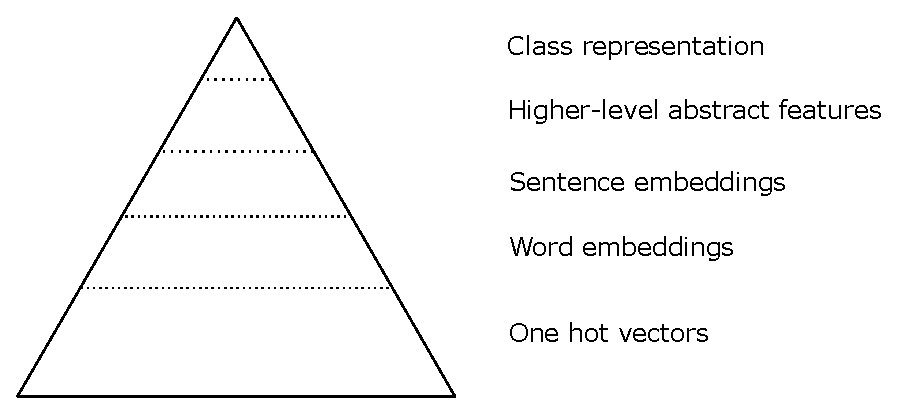
\includegraphics[width=13cm]{embedding_dim_red.eps}
	\centering
	\caption{A pyramid of abstraction of processing a natural language using neural networks}
	\label{embedding_dim_red_figure}
\end{figure}

\paragraph{}
In some cases, it might be beneficial to pre-train a part of the neural network in advance. For example, it is possible to pre-train word embeddings or a whole sentence encoder that is later used to build the final neural network. The pre-training can be done in a supervised as well as unsupervised way.

\section{Vector Representation of Words}\label{word_embedding}
\paragraph{}
An embedding of words can be directly useful for a lot of NLP tasks. Moreover, since sentences are made up of words, text representation techniques are often based on the word embeddings. The desired word representation is a low dimensional vector (about hundreds of dimensions) of real numbers that captures the semantics of the word. Put differently, it is expected that two similar words appear close to each other in a vector space of the representations. A favorable fact is that the embeddings can be trained using unsupervised learning on a large text corpus. Such techniques are usually based on a distributional hypothesis \cite{nlp_eisenstein}.

\paragraph{}
In this section, two types of word representations - context-free and contextual representations are presented. At the end of the section, a concept of subword models is also briefly discussed.

\subsection{Context-Free Word Representation}\label{context_free_embedding}
\paragraph{}
Context-free word representation techniques are identified by creating a fixed vector for each word, no matter its context. It means that, for example, the word "bank" would have the same representation when it appears in a context "bank account" as in case it appears in a context "river bank" \cite{bert_ithub}.

\paragraph{}
An advantage of this approach is that unlike the contextual representations, the word embedding is self-standing. Therefore, a similarity score of two words can be computed and used for similar word search.

\subsubsection{Word2Vec}\label{w2v}
\paragraph{}
A Word2Vec \cite{word2vec} is an unsupervised technique to represent words as vectors. Generally, this algorithm can be found in two forms. The first one is called a continuous bag of words (CBOW) and lies in predicting a target word given its context. The other method, on the contrary, predicts the context given a central word and is known as a skip-gram model. 

\paragraph{}
The skip-gram model is trained in a way that the central word is used as an input to a neural network that produces a conditional probability of the central word co-occurring next to other adjacent words in a sliding window. The window size defines the number of neighboring words taken into account. Then the vector representing the central word (which is stored in a weight matrix of the network) is adjusted to maximize the computed conditional probabilities for the neighboring words. The way how the CBOW model is trained is analogical and further explained in \cite{training_word2vec} together with mathematical details of the skip-gram model.

\subsubsection{Global Vectors (GloVe)}
\paragraph{}
Global Vectors (GloVe) \cite{glove} are another method of creating word embeddings. Unlike Word2Vec, GloVe utilizes a global word co-occurrence statistic that is captured in a co-occurrence matrix. To turn such a matrix into a vector representation, the authors introduced a new algorithm. It is based on optimizing the word vectors so that the dot product of the two word embeddings is equal to a logarithm of their co-occurrence count.

\subsection{Contextual Word Representation}
\paragraph{}
As stated in section \ref{context_free_embedding}, the context-free representations do not capture the context in which a word is used and this feature may be undesirable in many NLP tasks. Fortunately, contextual word representation techniques exist. The idea is that hidden layers in an LSTM based language model contain contextualized representations of fed-in words. The usage of such embeddings is then different than with the fixed representations, such as pre-trained Word2Vec (section \ref{w2v}). Instead of querying a lookup table, the vector embedding is obtained by passing the words into a model that produces the contextual embedding later used as an input to a task-specific neural network. An example of contextual word representations based on the deep bi-directional LSTM language model is ELMo (Embeddings from Language Models) \cite{elmo}.

\paragraph{}
Another contextual embedding method is a BERT \cite{bert} (Bidirectional Encoder Representations from Transformer) model. This model is based on Transformer architecture \cite{attention_is_all_you_need}, and its utilization provides outstanding results in many tasks.

\subsection{Subword Embedding}\label{subword_models}
\paragraph{}
A significant drawback of the techniques presented in section \ref{context_free_embedding} is that they are not able to handle uncommon and out of vocabulary words (OOVs) - word for which an embedding does not exist. Techniques trying to overcome this obstacle are called subword embeddings and are based on dividing words into smaller units down to a character level. For instance, the word "inevitable" can be composed of two units "in" and "evitable".

\subsubsection{Byte-Pair Encoding}\label{BPE}
\paragraph{}
A byte-Pair encoding \cite{nlp_stanford} is an unsupervised text segmentation algorithm which originated as a compression method. The algorithm starts with a list of elementary symbols, such as characters. Then it creates a new symbol composed of the most frequent symbol pair that appears in the training text. This step is repeated until the desired size of the vocabulary is achieved.

\subsubsection{WordPiece}
\paragraph{}
Another unsupervised method for subword tokenization is a WordPiece algorithm \cite{nlp_stanford}, which is to some extent similar to the Byte-Pair encoding (section \ref{BPE}). The difference is in the merging step. Instead of combining the two most frequent pairs, WordPiece chooses a couple, that would increase the log-likelihood of a language model \cite{nlp_eisenstein} if added to the vocabulary.

\section{Vector Representation of Sentences}\label{vector_representation_of_sentences}
\paragraph{}
As stated in the introduction of chapter \ref{vector_repr_chapter}, having a robust vector representation of text may be advantageous or even necessary for many NLP tasks. In this section, some of the used methods for obtaining semantic sentence embeddings are presented. 

\subsection{Combining Word Embeddings}\label{word_averaging}
\paragraph{}
Simple methods obtain a vector representation of text by combining pre-trained word vectors. One way how to combine the word embeddings is a summation or a weighted average, where the weights are tf-idf scores computed from a language corpus \cite{weighted_averaging_tfidf}. The tf-idf score for the $i$-th word is calculated according to equation \ref{tf_idf_eq}, where $k$ is the number of all words in the $j$-th document and $n_{xy}$ denotes an occurrence count of the $x$-th word in the $y$-th document. Finally $|D|$ is the number of documents in the corpora and  $|\{j:t_i \in d_j\}|$ is the number of documents where the word $i$ appears.

\begin{equation}
tf\_idf_i = \frac{n_{ij}}{\sum_{k}n_{kj}} * log \frac{|D|}{|\{j:t_i \in d_j\}|}
\label{tf_idf_eq}
\end{equation}  

\subsection{Supervised Representation Learning}\label{supervised_repre_learning}
\paragraph{}
A different way how to get a robust vector representation of text is to train a neural network model on a supervised learning task since the sentence embedding would then lie in hidden layers of the neural network. For example, in case of a network that consists of an embedding layer on the beginning, two LSTMs above it and two dense layers at the output, the representation of the sentence can be taken from the output of the second LSTM layer. A significant downturn of this method is a necessity of a labeled dataset that may not be available in many cases.

\paragraph{}
The quality of the embeddings obtained by this technique depends on the choice of a learning objective. Examples of such tasks are, for instance, machine translation or natural language entailment (section \ref{snli}). Another supervised learning objective is a semantic similarity task, which aims to recognize whether two texts are similar or not on a semantic basis. This task is going to be further focused by the rest of the work and a more detailed description can be found in section \ref{semantic_similarity_tasks}.

\subsection{Unsupervised Representation Learning}
\paragraph{}
In cases when a labeled dataset is not available, an unsupervised representation learning might come into play. Generally, a principle of the supervised representation learning (section \ref{supervised_repre_learning}) applies for the unsupervised case in the same way - the desired vector representation of sentences is in the hidden layers. The difference is the choice of the learning task, which is unsupervised in this case. 

\paragraph{}
To give an example, the BERT model \cite{bert} is trained on two unsupervised tasks. The first one is to predict a randomly masked token from an input sequence based on its context. The second one is the next sentence task, which aims to predict whether one sentence follows the other one in the original text. Another unsupervised learning model called GPT-2 \cite{GPT2} is trained on predicting the next word in a text.

\section{Semantic Similarity Task}\label{semantic_similarity_tasks}
\paragraph{}
In many real applications of the NLP, such as search engines, it is essential to measure or identify whether two texts are similar or not. Although this may look easy to accomplish just by looking if both documents contain the same keywords, distinguishing between tiny semantic nuances may be a severe problem. To differentiate texts with minor semantic differences is a target of a semantic similarity task, which is under ongoing research at the moment. Generally, the approach is to embed sentences into an $n$-dimensional space and then to compute a cosine similarity (equation \ref{cosine_similarity_eq}) or another metric of the two vectors. 

\begin{equation}
similarity = cos(\theta) = \frac{A \cdot B}{||A|| \: ||B||}
\label{cosine_similarity_eq}
\end{equation}

\paragraph{}
Therefore, the main objective of the semantic similarity task is to create embedding vectors that contain robust semantic information (section \ref{vector_representation_of_sentences}). The following sections present the related datasets and techniques.

\subsection{Related Datasets}\label{semantic_similarity_datasets}
\paragraph{}
For the semantic similarity task, there is not a lot of data available, which is a crucial problem in this field. While some datasets suffer from a small size, some of the others are partially made up of automatically generated samples, which may be undesirable as well. In this section, some of the available datasets are discussed.

\subsubsection{STS Benchmark}
\paragraph{}
STS benchmark dataset \cite{STSbenchmark} is a subset of data used in SemEval competitions. Examples contained in the dataset come from various sources such as user forums, image captions and news headlines. The dataset is separated into three subsets - training, development and testing. The total size of the dataset is around 8 600 samples and the sizes of the dataset parts are shown in table \ref{STSbenchmark_counts}.

\begin{table}[h!]
	\begin{center}
		\begin{tabular}{l r} 
			\hline
			\textbf{Dataset part} & \textbf{Dataset size} \\ [0.5ex] 
			\hline\hline
			training & 5 749 \\ 
			development & 1 500 \\
			testing & 1 379 \\ 
			\hline
		\end{tabular}
	\end{center}
	\caption{Sizes of training, development and testing parts of the STS Benchmark dataset.}
	\label{STSbenchmark_counts}
\end{table}

\subsubsection{Stanford Natural Language Inference Dataset}\label{snli}
\paragraph{}
A Stanford Natural Language Inference dataset (SNLI) \cite{snli} consists of human-labeled pairs of sentences. The possible labels are a contradiction, entailment, and neutral relationship. Although a learning objective of this dataset is not the semantic similarity, a natural language inference task requires a meaningful vector representation of sentences in the same way as the semantic similarity does. In other words, the significant difference lies in the classifier built over the representations. Thanks to that, the SNLI can be used for both an evaluation and training of the semantic representations of a text. 

\paragraph{}
The SNLI dataset, which consists of 570 000 examples, is split into three parts - training, development and testing. The sizes of these parts are shown in table \ref{SNLI_counts}. The amount of data and a lack of automatically generated examples make SNLI a very reasonable choice for many researchers. An example of the dataset pairs with the corresponding labels from the original paper \cite{snli} are shown in table \ref{SNLI_examples}.

\begin{table}[h!]
\begin{center}
	\begin{tabular}{l r} 
		\hline
		\textbf{Dataset part} & \textbf{Dataset size} \\ [0.5ex] 
		\hline\hline
		training & 550 152 \\ 
		development & 10 000 \\
		testing & 10 000 \\ 
		\hline
	\end{tabular}
\end{center}
\caption{Sizes of training, development and testing parts of the SNLI dataset.}
\label{SNLI_counts}
\end{table}

\begin{table}[h!]
	\begin{center}
		\begin{tabular}{p{5cm} p{5cm} p{2cm}} 
			\hline
			\textbf{Text} & \textbf{Hypothesis} & \textbf{Label} \\ [0.5ex] 
			\hline\hline
			A man inspects the uniform of a figure in some East Asian country. & The man is sleeping. & contradiction \\ 
			\hline
			An older and younger man smiling. & Two men are smiling and laughing at the cats playing on the floor. & neutral \\
			\hline
			A soccer game with multiple males playing. & Some men are playing a sport. & entailment \\ 
			\hline
		\end{tabular}
	\end{center}
	\caption{Three examples from the SNLI dataset.}
	\label{SNLI_examples}
\end{table}

\subsection{Related Work}\label{semantic_similarity_related_work}
\paragraph{}
Since the rest of the work focuses on the vector representation of text enriched with source code snippets, the following section presents an existing work on related topics. The paragraphs provide a brief description of the papers. A more detailed description can be found in the cited sources.

\subsubsection{A large annotated corpus for learning natural language inference}
\paragraph{}
Authors of the SNLI dataset published the results of three different models in their paper \cite{snli}. Generally, all of their models consist of a word embedding layer for both premise and hypothesis and a sentence embedding layers on the top of the word embeddings. In the end, classification is done by three 200-dimensional dense layers taking the 100-dimensional representation of the premise and hypothesis as an input. At the output, there is a softmax layer. A difference between these models is a method of sentence representation. The first and most simple model uses a sum of the word embeddings. The next one uses a simple RNN layer, whereas the last one uses an LSTM layer for sentence representation. The latest mentioned model is the most successful one with a test accuracy of $77.6\%$.

\subsubsection{Shortcut-Stacked Sentence Encoders for Multi-Domain Inference}
\paragraph{}
In 2017, Nie X. and Bansal M. presented their work on a Shortcut-Stacked Sentence Encoder \cite{shortcut_stacked_sentence_encoders}. It aims to represent a sentence as a vector of real numbers that is later used for an NLI classification. The model is made up of three bi-directional LSTM layers with shortcut connections and a classifier on top of it. The shortcut connections are made in the way that input of each LSTM layer consists of an original word embedding concatenated with a corresponding sequential output of all the preceding LSTMs. Such an approach led to an $86.0\%$ accuracy on the SNLI dataset.

\subsubsection{Sentence Embeddings in NLI with Iterative Refinement Encoders}
\paragraph{}
Another work \cite{HBMP} related to obtaining a vector representation of text introduces a hierarchical structure of bi-directional LSTM layers that implements an iterative reinforcement strategy. The key idea behind the model is that each subsequent LSTM layer is initialized with the last hidden state of the preceding layer while accepting the original word embeddings as an input. An output of each LSTM is then max-pooled and concatenated to a resulting representation. The authors have reported a very good accuracy of $86.6\%$ on the SNLI dataset.


\subsubsection{Dynamic Self-Attention Model}
\paragraph{}
Yoon D., Lee D. and Lee S. in their paper \cite{DSA} presented a new Dynamic Self-Attention (DSA) model, which outperforms many related models. DSA is based on attending to a dynamic weight vector rather than to a fixed vector learned during training. The model succeeded on the SNLI dataset with a result of $87.4\%$, which is the highest score among reported results in a sentence vector-based group of models.

\subsubsection{Semantics-aware BERT for Language Understanding}
\paragraph{}
At the moment, the best reported result on the SNLI dataset is achieved by a model called Semantic-aware BERT (SemBERT) \cite{semBERT}. It is a BERT \cite{bert} model extended by information about a semantic role of different parts of an input. More precisely, the BERT model is used to compute a contextual representation of word tokens. It is then concatenated with a vector, which carries the information about the semantic role of the token in a particular sentence. An achieved accuracy on the SNLI dataset is $91.9\%$.
 
\subsubsection{Retrieval on Source Code: A Neural Code Search}
\paragraph{}
In their paper, Sachdev S. et al. \cite{facebook0_unsupervised} addresses a natural language search over a large code base acquired from the GitHub. They use a variant of a Word2Vec embedding (section \ref{w2v}) to obtain a representation of the query and a code snippet. Three methods of creating a document embedding based on the word representations are evaluated. These are simple averaging of all the word vectors, averaging unique words only and a weighted average using the tf-idf (equation \ref{tf_idf_eq}). Such embedding of the query is then used to find a code snippet with its representation closest to the query embedding. The accuracy of the code search was evaluated on 100 hand-picked StackOverflow questions with an accepted answer. The most promising result is achieved using the weighted average method, where an acceptable solution was found for 43 out of 100 test queries.

\subsubsection{When Deep Learning Met Code Search}
\paragraph{}
Another existing work \cite{facebook1_supervised} extends the previously discussed method by introducing supervision into the training. A significant difference is that the authors use two different embedding matrices (the first one is used for the code and the second for the query), initialized by the same pre-trained weights. These matrices are then fine-tuned during the training process. Additionally, the scheme of producing a document level embedding from the word token embeddings is changed. Instead of the tf-idf weighted average, a simple average is used for the query and a weighted average based on learned attention weights is used for the code. 
